\documentclass[12pt,letterpaper]{exam}
\usepackage[lmargin=1in,rmargin=1in,tmargin=1in,bmargin=1in]{geometry}
\usepackage{../style/exams}

% -------------------
% Course & Exam Information
% -------------------
\newcommand{\course}{MAT 101: Exam 4}
\newcommand{\term}{Fall -- 2022}
\newcommand{\examdate}{12/14/2022}
\newcommand{\timelimit}{85 Minutes}

\setbool{hideans}{true} % Student: True; Instructor: False

% -------------------
% Content
% -------------------
\begin{document}

\examtitle
\instructions{Write your name on the appropriate line on the exam cover sheet. This exam contains \numpages\ pages (including this cover page) and \numquestions\ questions. Check that you have every page of the exam. Answer the questions in the spaces provided on the question sheets. Be sure to answer every part of each question and show all your work.} 
\scores
%\bottomline
\newpage

% ---------
% Questions
% ---------
\begin{questions}

% Question 1
\newpage
\question[10] Sketch the function $y= (x + 6)^2 - 7$ as accurately as possible on the graph below. Your sketch should include the vertex and axis of symmetry. 
	\[
	\fbox{
	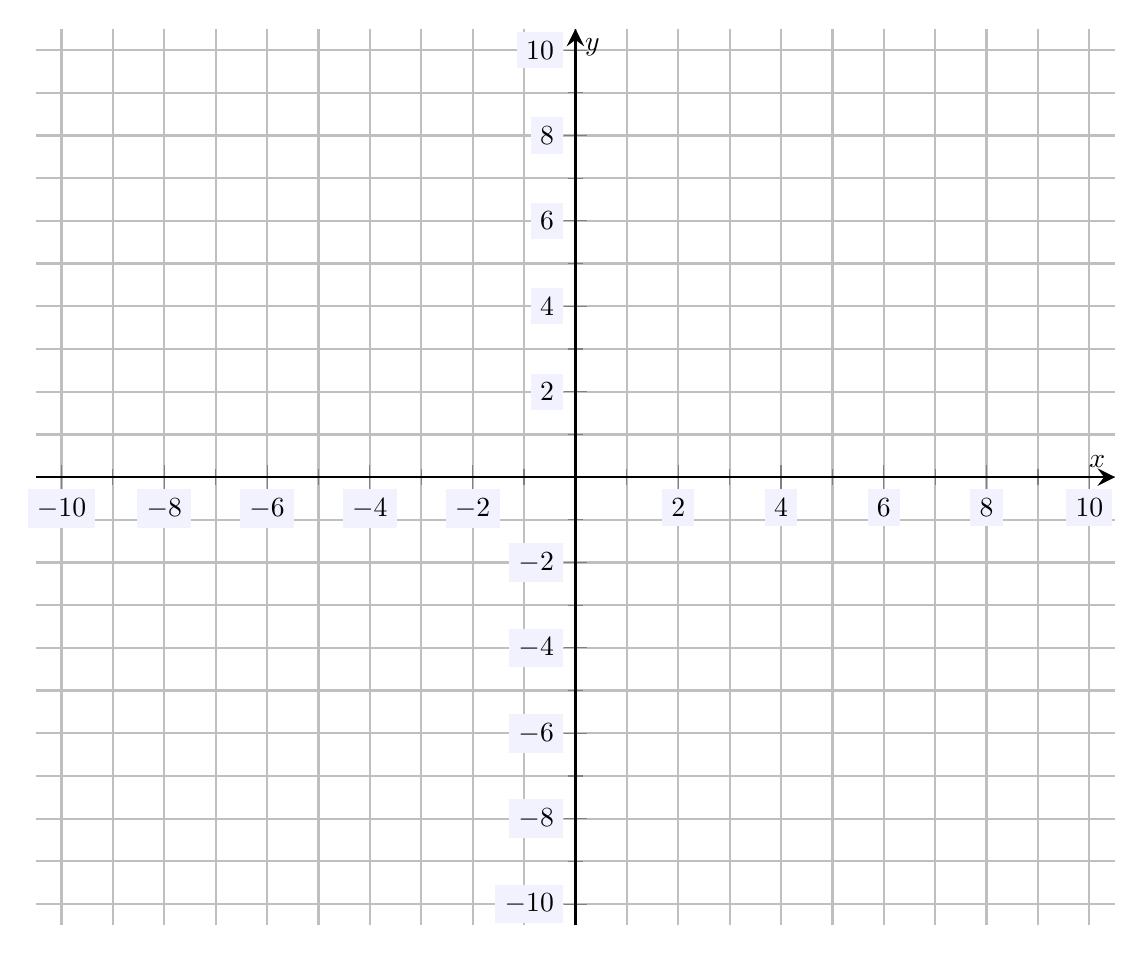
\begin{tikzpicture}[scale=2,every node/.style={scale=0.5}]
	\begin{axis}[
	grid=both,
	axis lines=middle,
	ticklabel style={fill=blue!5!white},
	xmin= -10.5, xmax=10.5,
	ymin= -10.5, ymax=10.5,
	xtick={-10,-8,-6,-4,-2,0,2,4,6,8,10},
	ytick={-10,-8,-6,-4,-2,0,2,4,6,8,10},
	minor tick = {-10,-9,...,10},
	xlabel=\(x\),ylabel=\(y\),
	]
%	\draw[line width= 0.03cm, dotted] (-6,-10.5) -- (-6,10.5);
%	\addplot[samples= 100, domain= -10.5:0, line width= 0.03cm] ({x}, {(x + 6)^2 - 7});
%	\draw[fill=black] (-6,-7) circle (0.2);
	\end{axis}
	\end{tikzpicture}
	}
	\]



% Question 2
\newpage
\question[10] A quadratic function $f(x)= ax^2 + bx + c$ is plotted below. Find $a$, $b$, and $c$ for this function. 
	\[
	\fbox{
	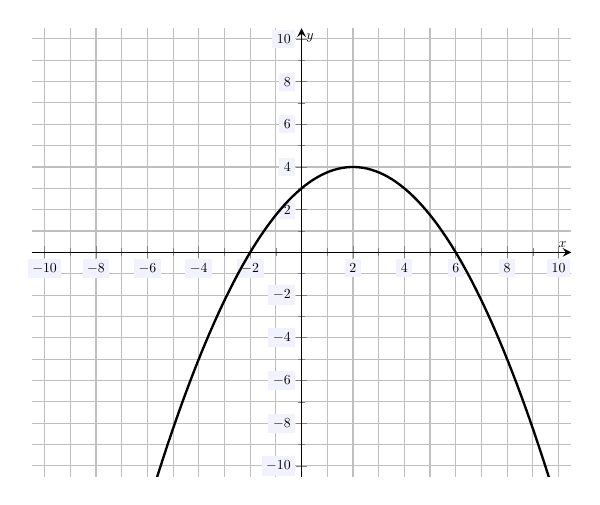
\begin{tikzpicture}[scale=1,every node/.style={scale=0.5}]
	\begin{axis}[
	grid=both,
	axis lines=middle,
	ticklabel style={fill=blue!5!white},
	xmin= -10.5, xmax=10.5,
	ymin= -10.5, ymax=10.5,
	xtick={-10,-8,-6,-4,-2,0,2,4,6,8,10},
	ytick={-10,-8,-6,-4,-2,0,2,4,6,8,10},
	minor tick = {-10,-9,...,10},
	xlabel=\(x\),ylabel=\(y\),
	]
	\addplot[samples= 100, domain= -6:10, line width= 0.03cm] ({x}, {-1/4*(x - 2)^2 + 4});
	\end{axis}
	\end{tikzpicture}
	}
	\]



% Question 3
\newpage
\question[10] Consider the quadratic function $f(x)= \dfrac{5}{3} - \left(x + \dfrac{3}{2} \right)^2$.
	\begin{enumerate}[(a)]
	\item Find the vertex and axis of symmetry for $f(x)$.
	\item Does this parabola open upwards or downwards?
	\item Is this parabola concave or convex?
	\item Does this parabola have a maximum or minimum? 
	\item Find the maximum or minimum of $f(x)$, if it exists. 
	\end{enumerate}



% Question 4
\newpage
\question[10] Showing all your work, find the vertex form of $f(x)= 4x^2 + 4x - 6$. 



% Question 5
\newpage
\question[10] Find the $y$ and $x$-intercepts for the function $f(x)= x^2 + 21x - 72$. 



% Question 6
\newpage
\question[10] Use the discriminant of $f(x)= x^2 - 3x - 108$ to show that $f(x)$ has a `nice' factorization and then find its factorization. 



% Question 7
\newpage
\question[10] Use the discriminant of some quadratic function to show that the equation given below does not have a `nice' solution.
	\[
	31= x(14 - x)
	\]



% Question 8
\newpage
\question[10] Showing all your work, factor the polynomial $x^2 - 23x - 24$. Verify that your factorization is correct. 



% Question 9
\newpage
\question[10] Showing all your work, factor the polynomial $x^2 + 17x - 84$. 



% Question 10
\newpage
\question[10] Showing all your work, factor the polynomial $7x^2 + 18x - 9$. 



% Question 11
\newpage
\question[10] Showing all your work, use the quadratic formula to factor the polynomial $288x^2 - 1524x + 935$. 



% Question 12
\newpage
\question[10] Showing all your work, solve the equation below then verify that your solution(s) are correct:
	\[
	x^2 + 9= 10x
	\]



% Question 13
\newpage
\question[10] Showing all your work, solve the equation below:
	\[
	6x^2= 5 - 7x
	\]



% Question 14
\newpage
\question[10] Showing all your work, solve the equation below:
	\[
	-x^2= 2(23 - 7x)
	\]


\end{questions}
\end{document}